\documentclass[12pt,a4paper]{report}

\usepackage[brazil]{babel}
\usepackage[utf8]{inputenc}

\usepackage{graphicx}

\title{Especificações do Projeto SIGEST}
\author{Taciano Morais Silva - tacianosilva@gmail.com}

\begin{document}

\maketitle
\listoffigures
\tableofcontents

\chapter{Introdução}

Texto de introdução para testar a citação \cite{morais04a}.

\section{Definição de Perfis}

No sistema teremos vários tipos de usuário e seus respectivos perfis.
Segue abaixo a lista de usuários do sistema e seus respecitivos perfis. 

\emph{Professor} - Entidade que representa o professor que pode assumir um dos
seguintes perfis:

\begin{itemize}
\item Coordenador de Curso
\item Coordenador de Estágio
\item Avaliador de Estágio
\item Orientador de Estágio
\end{itemize}

\emph{Administrador} - Entidade que representa o super usuário que pode
assumir um dos seguintes perfis:

\begin{itemize}
\item Administrador
\item Super Administrador
\end{itemize}

\chapter{Projeto Arquitetural}

\chapter{Modelo de Dados}

% Figura Modelo de Dados
\begin{figure}[!htb]
        \centering
        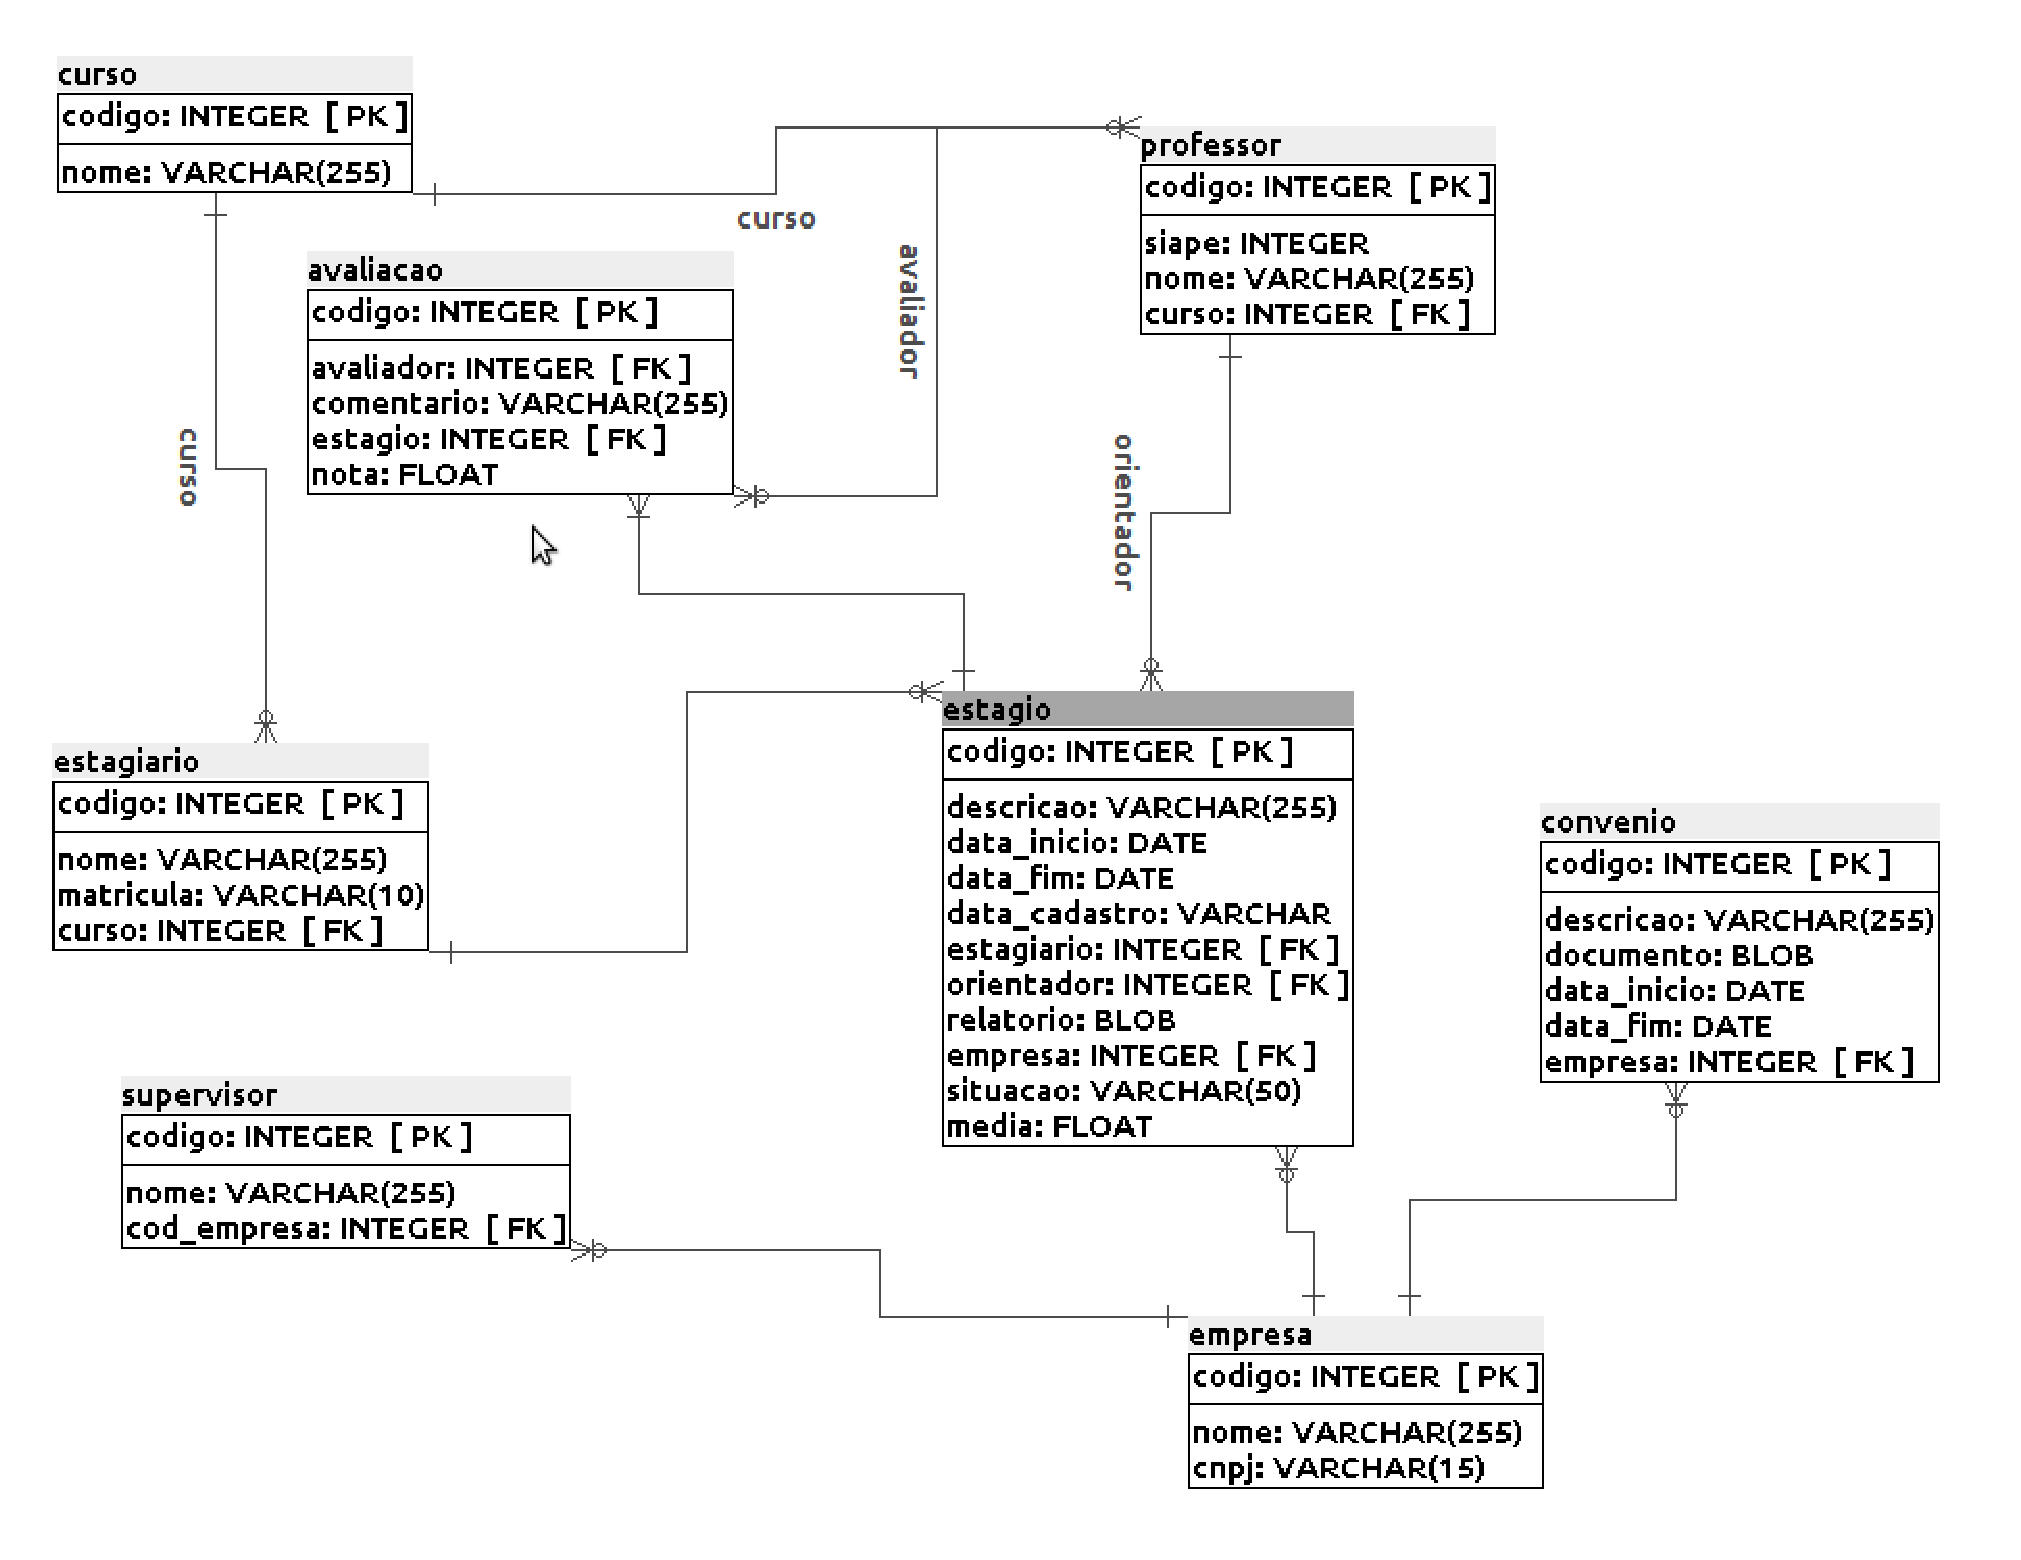
\includegraphics[scale=0.4]{esquema_sigest.eps}
        \caption{Esquema Relacionado para o Sistema SIGEST}
        \label{esquema_sigest}
\end{figure}
%\footnote{"A framework is a set of classes that embodies an abstract design for solutions to a family of related problems", \cite{johnson88}}


\chapter{Lista de Casos de Uso}

%% Input para a Section CDU001 - Estagiário
\section{CDU01 - Estagiário}

\subsection{Responsável}

Nome: Fladson

GitHub:

\subsection{Descrição}

\subsection{Fluxo Principal}

\subsection{Fluxo Secundário}

\subsection{Fluxo de Exceção}

\subsection{Diagrama de Classe}

\subsection{Diagrama de Sequência}

\section{CDU02 - Estágio}

\subsection{Responsável}

Nome: Aragon

GitHub:

\subsection{Descrição}

\subsection{Fluxo Principal}

\subsection{Fluxo Secundário}

\subsection{Fluxo de Exceção}

\subsection{Diagrama de Classe}

\subsection{Diagrama de Sequência}

\section{CDU03 - Empresa}

\subsection{Responsável}

Nome: Alisson

GitHub:

\subsection{Descrição}

\subsection{Fluxo Principal}

\subsection{Fluxo Secundário}

\subsection{Fluxo de Exceção}

\subsection{Diagrama de Classe}

\subsection{Diagrama de Sequência}

\section{CDU04 - Professor}

\subsection{Responsável}

Nome: Mércia

GitHub:

\subsection{Descrição}

\subsection{Fluxo Principal}

\subsection{Fluxo Secundário}

\subsection{Fluxo de Exceção}

\subsection{Diagrama de Classe}

\subsection{Diagrama de Sequência}

%%%%%%%%%%%%%%%%%%%%%%%%%%%%%%%%%%%%%%%%%%%%%%%%%%%%%%%%%%%%%%%%%%%%%%%%%%%%%%%
%% Bibliografia

\bibliographystyle{alpha} % estilo de bibliografia
\bibliography{bib-dis} % arquivos com as entradas bib.

%%%%%%%%%%%%%%%%%%%%%%%%%%%%%%%%%%%%%%%%%%%%%%%%%%%%%%%%%%%%%%%%%%%%%%%%%%%%%%%
%% Ap\^endice
 % Caso seja necessário algum apêndice, descomente a próxima linha.

%\appendix

%\input{capA-filosofos}

\end{document}
